%TODO:
% Introduzione dove spieghi un po' in generale il problema 
% che hai affrontato (segmentazione automatica di un oggetto
% su immagini di ecografie) e l'obiettivo.


% \section{Introduzione}
\chapter{Introduzione} % (fold)
\label{chap:Introduzione}

% chapter Introduzione (end)


\section{Binary Semantic Segmentation}

La segmantazione semantica è una tecnica di \textit{computer vision} che permette di assegnare ad ogni pixel di un'immagine un'etichetta che ne descrive il contenuto.

\begin{figure}[!ht]
	\begin{adjustbox}{width=0.8\columnwidth, center}
		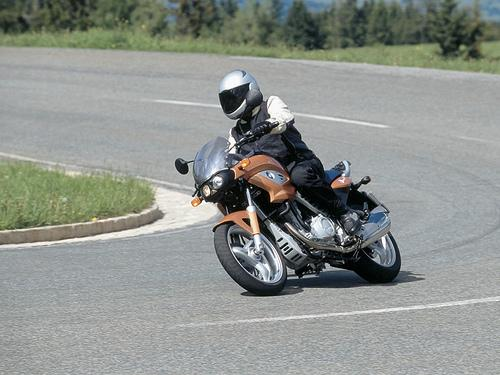
\includegraphics{./images/segmantion_example_image.png}
    \hspace{20pt} % Add horizontal space between the two images
    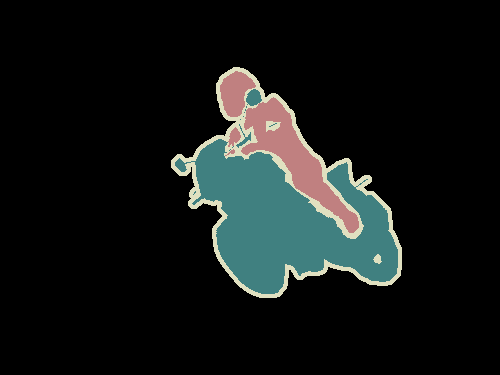
\includegraphics{./images/segmantion_example_mask.png}
	\end{adjustbox}
	\caption{Segmentazione semantica (Fonte: \cite{pascal-voc-2012})}
	\label{fig:segmantion_example}
\end{figure}

Nello specifico in questa tesi si tratta una sottocategoria della semganzione semantica,
ovvero la \textbf{Binary Semantic Segmentation}(segmentazione semantica
binaria), questa tecnica di \textit{computer vision} permette di assegnare ad ogni pixel
di un'immagine un'etichetta che ne descrive il contenuto, ma a differenza della
segmentazione semantica classica, che permette di assegnare ad ogni pixel una delle $N$
possibili etichette, la segmentazione semantica binaria permette di assegnare ad ogni
pixel una delle due etichette possibili: \textbf{oggetto} o \textbf{sfondo}.

La segmentazione \`e una tipologia di problema molto ricorrente in ambito medico,
in quanto permette di automatizzare alcune procedure che altrimenti sarebbero
eseguite manualmente, riducendo i tempi di esecuzione e i costi,
permettendo di ottenere risultati pi\`u precisi e accurati limitando lo sforzo umano.


\section{Fully Convolutional Network}

Le \textbf{Fully Convolutional Network} (FCN) \cite{long2015fully} sono una tipologia di reti neurali convoluzionali (CNN) che permettono di effettuare segmentazioni semantiche, in quanto sono in grado di gestire input di qualsiasi dimensione e di produrre mappe di segmentazione pi\`u precise grazie alla loro capacit\`a di apprendere contesti spaziali.


\begin{figure}[!ht]
	\begin{adjustbox}{width=0.6\columnwidth, center}
		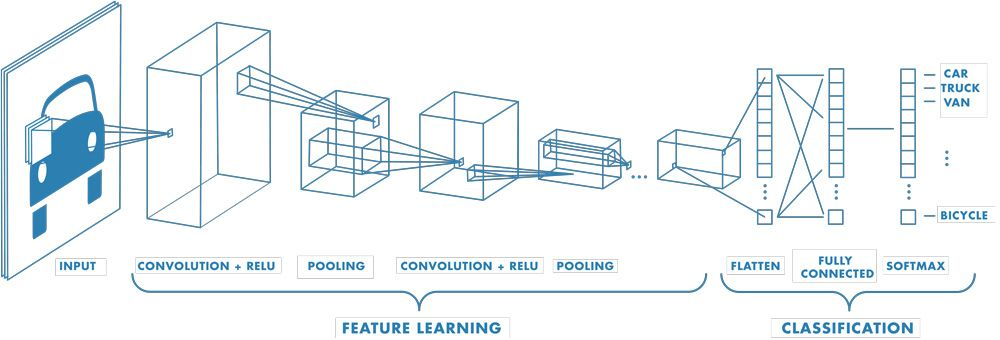
\includegraphics{./images/cnn.png}
	\end{adjustbox}
	\caption{CNN (Fonte: \cite{cnn_example})}
	\label{fig:cnn}
\end{figure}

Le motivazioni riguardanti l'ampio utilizzo nel settore della \textit{computer vision}
sono legate all'assenza di strati completamente connessi (lineari) che vincolano
l'input alla medesima grandezza per ogni singola immagine, permettendo di fornire in input l'intera immagine e non frammenti della stessa così da aumentare l'apprendimento spaziale della rete.

Questa maggior flessibilità comporta un'addestramento libero da limitaioni sull'input comportando una maggiore tolleranza agli errori e al rumore rendendo questa tipologia di reti particolarmente adatte a contesti poveri di dati.


\section{U-Net}

L'architettura \textbf{U-net} \cite{ronneberger2015unet} è una particolare implementazione di FCN che permette di effettuare segmentazioni semantiche, in quanto è in grado di gestire input di qualsiasi dimensione e di produrre mappe di segmentazione pi\`u precise grazie alla sua capacit\`a di apprendere contesti spaziali.


\begin{figure}[!ht]
	\begin{adjustbox}{width=0.6\columnwidth, center}
		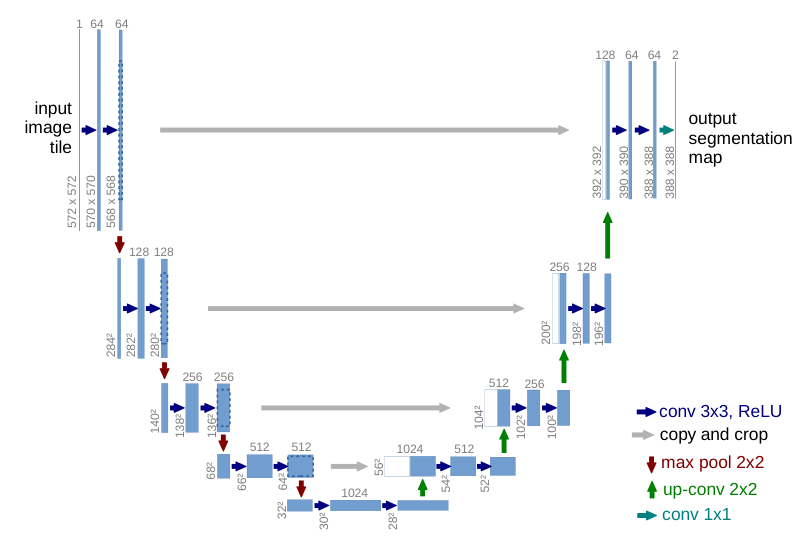
\includegraphics{./images/unet.png}
	\end{adjustbox}
	\caption{U-Net (Fonte: \cite{ronneberger2015unet})}
	\label{fig:unet}
\end{figure}




%
%
%
%
%
